%
%===============>>  ГРУППА 9-1 МОДУЛЬ 4  <<=============
%
\setmodule{4}
%
%===============>>  Занятие 1  <<===============
%
\begin{class}[number=1]
	\begin{listofex}
		\item Вычислить рациональным способом:
		\begin{enumcols}[itemcolumns=3]
			\item \( \sqrt{16+4\cdot4\cdot24} \)
			\item \( \sqrt{83^3\cdot2^2-83^2\cdot2^3} \)
			\item \( \sqrt{50^2-4\cdot7\cdot7} \)
		\end{enumcols}
		\item Построить график функции \( y=2x-5 \).
		\begin{enumcols}[itemcolumns=1]
			\item Проверить \textit{(графическим, а потом аналитическим способом)}, принадлежит ли точка с координатами \( (4;3) \) графику этой функции?
			\item Принадлежит ли точка с координатами \( (112;217) \) графику этой функции?
			\item Найти точку пересечения графика данной функции с графиком функции \( y=4x-1 \).
		\end{enumcols}
		\item Построить график функции \( f(x)=x^2-2x+1 \). Выберите верные утверждения:
		\begin{enumcols}[itemcolumns=1]
			\item График функции возрастает на промежутке \( [0;+\infty) \);
			\item График функции убывает на промежутке \( [-5;-2] \);
			\item \( f(-1)>f(1) \);
			\item \( f(x)=4 \) при \( x=3 \);
			\item Наименьшее значение функция принимает при \( x=-1 \);
			\item При \( x=2 \) значение функции больше чем при \( x=0 \);
			\item \( f(-1)=f(3) \);
			\item Корнем уравнения \( f(x)=9 \) является только \( x=-2 \);
			\item \( f(x)\ge0 \) при любом \( x \);
			\item Данный график функции пересекается с графиком \( y=-2x+5 \) в одной точке.
		\end{enumcols}
		\item Решить систему неравенств:
		\[ \left\{
		\begin{array}{l}
			3(x-1)-2(2-3x)>5x-3,\\
			8x-3(2x+5)<2(x-7).
		\end{array}
		\right. \]
		\item При каких значениях переменной выражение \( \sqrt{4x+1}+\sqrt{2-3x} \) имеет смысл?
		\item Построить график функции \( y=x-|2x+1|-2 \). Найти точки пересечения данного графика с графиком функции \( y=x-5 \).
	\end{listofex}
\end{class}
%
%===============>>  Занятие 2  <<===============
%
\begin{class}[number=2]
	\begin{listofex}
		\item Из закона всемирного тяготения \( F=G\cdot\dfrac{mM}{r^2} \) выразите массу \( m \) и найдите ее величину (в килограммах), если \( F=13,4 \) H, \( r=5 \) м, \( M=5\cdot10^9 \) и гравитационная постоянная \( G=6,7\cdot10^{-11} \) \( \dfrac{\text{м}^3}{\text{кг}\cdot\text{с}^2} \).
		\item Известно, что \( c<-1 \). расположите в порядке убывания числа \( c,\; c^2,\; \dfrac{1}{c}\).
		\begin{enumcols}[itemcolumns=4]
			\item \( c^2,\; c,\; \dfrac{1}{c} \)
			\item \( c^2,\; \dfrac{1}{c},\; c \)
			\item \( c,\; c^2,\; \dfrac{1}{c} \)
			\item \( c,\; \dfrac{1}{c},\; c^2 \)
		\end{enumcols}
		\item Какое из данных чисел принадлежит отрезку \( [3;4] \)?
		\begin{enumcols}[itemcolumns=4]
			\item \( \dfrac{45}{19} \)
			\item \( \dfrac{52}{19} \)
			\item \( \dfrac{68}{19} \)
			\item \( \dfrac{77}{19} \)
		\end{enumcols}
		\item Постройте графики функции \( y=4x-1 \) и \( y=-\dfrac{1}{2}x+2,5 \). Графически определите точку пересечения этих графиков. Во сколько раз ордината точки пересечения больше абсциссы?
		\item Найдите точку пересечения графиков функций \( y=12x-70 \) и \( y=6x+2 \).
		\item Постройте график функции \( f(x)=x^2-6x+8 \). Выберите верные утверждения:
		\begin{enumcols}[itemcolumns=1]
			\item График функции возрастает на промежутке \( [4;+\infty) \);
			\item График функции убывает на промежутке \( [-7;7] \);
			\item \( f(-4)<f(4) \);
			\item \( f(x)=5 \) при \( x=0 \);
			\item Данная функция имеет максимальное значение при \( x=9 \);
			\item При \( x=-2 \) значение функции больше чем при \( x=0 \);
			\item \( f(-1)=f(3) \);
			\item \( f(x)\ge0 \) при \( x\ge4 \);
			\item \( f(x)\ge0 \) только при \( x\ge4 \);
			\item Данный график функции пересекается с графиком \( y=-x-8 \) в двух точках.
		\end{enumcols}
		\item Подставьте вместо знака \( * \) число так, чтобы функция \( y=2x^2-3x+* \) проходила через точку с координатами \( (4;15) \).
		\item Решить систему неравенств:
		\[ \left\{
		\begin{array}{l}
			6(x+2)-4(0,5-2x)>2x-6,\\
			9x+x(2x+5)<2(x^2-7).
		\end{array}
		\right. \]
		\item При каких значениях переменной выражение \( \sqrt{12x-6}+\sqrt{4-5x} \) имеет смысл?
		\item Высота равностороннего треугольника равна \( 15\sqrt{3} \). Найдите его периметр.
	\end{listofex}
\end{class}
%
%===============>>  Домашняя работа 1  <<===============
%
%\begin{homework}[number=1]
%	\begin{listofex}
%		\item Пусто
%	\end{listofex}
%\end{homework}
%
%===============>>  Занятие 3  <<===============
%
\begin{class}[number=3]
	\begin{listofex}
			\item 
			\begin{minipage}[t]{0.57\textwidth}
				Найдите значение \( a \) по графику функции \( y=ax^2+bx+c \), изображенному на рисунке.
			\end{minipage}
			\begin{minipage}[c]{0.3\textwidth}
				
\includegraphics[align=t, width=\textwidth]{pics/G91M4L4-1}
			\end{minipage}
		
				\item 
			\begin{minipage}[t]{0.57\textwidth}
				Найдите значение \( k \) по графику функции \( y=\dfrac{k}{x} \), изображенному на рисунке.
			\end{minipage}
			\begin{minipage}[c]{0.3\textwidth}
			
\includegraphics[align=t, width=\textwidth]{pics/G91M4L4-1}
		\end{minipage}
		\begin{enumcols}[itemcolumns=4]
			\item \( 2 \)
			\item \( \dfrac{1}{2} \)
			\item \( -\dfrac{1}{2} \)
			\item \( -2 \)
		\end{enumcols}
	
		\item 
		\begin{minipage}[t]{0.57\textwidth}
			На рисунке изображён график квадратичной функции \( y=f(x) \). Какие из следующих утверждений о данной функции неверны? Запишите их номера.
		\end{minipage}
		\begin{minipage}[c]{0.3\textwidth}
			
\includegraphics[align=t, width=\textwidth]{pics/G91M4L4-1}
		\end{minipage}
		\begin{enumcols}[itemcolumns=1]
			\item \( f(-1)=f(3) \)
			\item Наибольшее значение функции равно \( 3 \).
			\item \( f(x)>0 \) при \( -1<x<3 \)
		\end{enumcols}
	
		\item 
		\begin{minipage}[t]{0.57\textwidth}
			Установите соответствие между графиками функций и формулами, которые их задают. 
			\[ФУНКЦИИ\]
			\begin{enumcols}[itemcolumns=1]
				\item \( y=x^2 \)
				\item \( y=\dfrac{x}{2} \)
				\item \( y=\sqrt{x} \)
				\item \( y=\dfrac{2}{x} \)
			\end{enumcols}
		\end{minipage}
		\begin{minipage}[c]{0.3\textwidth}
			
\includegraphics[align=t, width=\textwidth]{pics/G91M4L4-1}
		\end{minipage}
		\begin{center}
			\footnotesize
			\begin{tabular}{|c|c|c|}
				\hline
				А&Б&В\\
				\hline
			 & & \\
			 \hline
			\end{tabular}
		\end{center}
	
		\item 
		\begin{minipage}[t]{0.57\textwidth}
			График какой из приведенных ниже функций изображен на рисунке?
		\end{minipage}
		\begin{minipage}[c]{0.3\textwidth}
			
\includegraphics[align=t, width=\textwidth]{pics/G91M4L4-1}
		\end{minipage}
		\begin{enumcols}[itemcolumns=4]
			\item \( y=-\dfrac{5}{x} \)
			\item \( y=-\dfrac{1}{5x} \)
			\item \( y=\dfrac{5}{x} \)
			\item \( y=\dfrac{1}{5x} \)
		\end{enumcols}
	
		\item 
		\begin{minipage}[t]{0.57\textwidth}
			Установите соответствие между функциями и их графиками.
			\[ФУНКЦИИ\]
			\begin{enumcols}[itemcolumns=3]
				\item \( y=-2x+4 \)
				\item \( y=2x-4 \)
				\item \( y=2x+4 \)
			\end{enumcols}
			\[ГРАФИКИ\]	
		\end{minipage}
		\begin{minipage}[c]{0.3\textwidth}
			
\includegraphics[align=t, width=\textwidth]{pics/G91M4L4-1}
		\end{minipage}
		\begin{center}
			\footnotesize
			\begin{tabular}{|c|c|c|}
				\hline
				А&Б&В\\
				\hline
			 & & \\
				\hline
			\end{tabular}
		\end{center}

		\item 
		\begin{minipage}[t]{0.57\textwidth}
			Установите соответствие между функциями и их графиками. 
			\[ФУНКЦИИ\]
			\begin{enumcols}[itemcolumns=3]
				\item \( y=\dfrac{1}{9x} \)
				\item \( y=\dfrac{9}{x} \)
				\item \( y=-\dfrac{9}{x} \)
			\end{enumcols}
			\[ГРАФИКИ\]	
		\end{minipage}
		\begin{minipage}[c]{0.3\textwidth}
			
\includegraphics[align=t, width=\textwidth]{pics/G91M4L4-1}
		\end{minipage}
			\begin{center}
				\footnotesize
				\begin{tabular}{|c|c|c|}
					\hline
					А&Б&В\\
					\hline
				 & & \\
					\hline
				\end{tabular}
			\end{center}
		
		\item 
		\begin{minipage}[t]{0.57\textwidth}
			Установите соответствие между графиками функций и формулами, которые их задают.
		\end{minipage}
		\begin{minipage}[c]{0.3\textwidth}
			
\includegraphics[align=t, width=\textwidth]{pics/G91M4L4-1}
		\end{minipage}
		\begin{enumcols}[itemcolumns=4]
			\item \( y=2x \)
			\item \( y=-2x \)
			\item \( y=x+2 \)
			\item \( y=2 \)
		\end{enumcols}
		\begin{center}
			\footnotesize
			\begin{tabular}{|c|c|c|}
				\hline
				А&Б&В\\
				\hline
			 & & \\
				\hline
			\end{tabular}
		\end{center}
	
		\item 
		\begin{minipage}[t]{0.57\textwidth}
			Установите соответствие между графиками функций и формулами, которые их задают.
		\end{minipage}
		\begin{minipage}[c]{0.3\textwidth}
			
\includegraphics[align=t, width=\textwidth]{pics/G91M4L4-1}
		\end{minipage}
		\begin{enumcols}[itemcolumns=1]
			\item \( y=-2x^2+6x-6 \)
			\item \( y=-2x^2-6x-6 \)
			\item \( y=2x^2+6x+6 \)
			\item \( y=2x^2-6x-6 \)
		\end{enumcols}
		\begin{center}
			\footnotesize
			\begin{tabular}{|c|c|c|}
				\hline
				А&Б&В\\
				\hline
			 & & \\
				\hline
			\end{tabular}
		\end{center}
	
		\item Период колебания математического маятника \( T \) (в секундах) приближенно можно вычислить по формуле \( T=2\sqrt{l} \), где \( l \) -- длина нити (в метрах). Пользуясь этой формулой, найдите длину нити маятника (в метрах), период колебаний которого составляет \( 3 \) секунды.
		
		\item Альпинисты в первый день восхождения поднялись на высоту \( 1400 \) м, а затем каждый следующий день поднимались на высоту на \( 100 \) м меньше, чем в предыдущий. За сколько дней они покорили высоту \( 5000 \) м?
		
		\item Для асфальтирования участка длиной \( 99 \) м используются \( 2  \) катка. Первый каток был установлен в одном конце участка, второй -- в противоположном. Работать они начали одновременно. Первый каток в каждую минуту проходил \( 5 \) м, а второй каток за первую минуту прошел \( 1,5 \) м, а за каждую следующую минуту проходил на \( 0,5 \) м больше, чем за предыдущую. Через сколько минут катки встретились?
		
		\item Занятия йогой начинают с \( 15 \) минут в день и увеличивают на \( 10 \) минут время каждый следующий день. Сколько дней следует заниматься йогой в указанном режиме, чтобы суммарная продолжительность занятий составила \( 2 \) часа?
		
		\item При свободном падении тело прошло в первую секунду \( 5 \) м, а в каждую следующую на \( 10 \) м больше. Найдите глубину шахты, если свободно падающее тело достигло его дна через \( 5 \) с после начала падения.
		
		\item Рихарду необходимо разобрать \( 315 \) квадратных уравнений. Ежедневно он разбирает на одно и то же количество уравнений больше по сравнению с предыдущем днём. Известно, что за первый день Рихард разобрал \( 11 \) квадратных уравнений, а справился со всеми он за \( 9 \) дней. Сколько уравнений Рихард разберёт в последний день?
		
		\item Клиент взял в банке кредит \( 100 \) рублей на n месяцев с условием, что по окончании первого месяца выплатит банку \( \dfrac{1}{n} \) часть кредита, а в каждый последующий месяц выплата будет на 5 рублей больше, чем в предыдущий. Известно, что в последний месяц выплата составила \( 55 \) руб. На какой срок был выдан кредит, если известно, что этот срок превышал полгода?
		\item 
		\begin{minipage}[t]{0.57\textwidth}
			При хранении бревен их укладывают, как показано на рисунке. Сколько бревен находится в одной кладке, если в ее основании положено \( 12 \) бревен?
		\end{minipage}
		\begin{minipage}[c]{0.3\textwidth}
			
\includegraphics[align=t, width=\textwidth]{pics/G91M4L4-1}
		\end{minipage}
	
		\item В амфитеатре 13 рядов. В первом ряду 17 мест, а в каждом следующем на 2 места больше, чем в предыдущем. Сколько всего мест в амфитеатре?
		
		\item 
		\begin{minipage}[t]{0.57\textwidth}
			Площадь ромба равна \( 54 \), а периметр равен \( 36 \). Найдите высоту ромба.
		\end{minipage}
		\begin{minipage}[c]{0.3\textwidth}
			
\includegraphics[align=t, width=\textwidth]{pics/G91M4L4-1}
		\end{minipage}
		
		\item 
		\begin{minipage}[t]{0.57\textwidth}
			Сторона ромба равна \( 4 \), а один из углов этого ромба равен \( 150\degree \). Найдите высоту этого ромба.
		\end{minipage}
		\begin{minipage}[c]{0.3\textwidth}
			
\includegraphics[align=t, width=\textwidth]{pics/G91M4L4-1}
		\end{minipage}
		
		\item 
		\begin{minipage}[t]{0.57\textwidth}
			Тангенс острого угла прямоугольной трапеции равен \( \dfrac{5}{6} \).  Найдите её большее основание, если меньшее основание равно высоте и равно \( 15 \).
		\end{minipage}
		\begin{minipage}[c]{0.3\textwidth}
			
\includegraphics[align=t, width=\textwidth]{pics/G91M4L4-1}
		\end{minipage}
		
		\item 
		\begin{minipage}[t]{0.57\textwidth}
			Основания трапеции равны \( 4 \) и \( 10 \). Найдите больший из отрезков, на которые делит среднюю линию этой трапеции одна из её диагоналей.
		\end{minipage}
		\begin{minipage}[c]{0.3\textwidth}
			
\includegraphics[align=t, width=\textwidth]{pics/G91M4L4-1}
		\end{minipage}
	\end{listofex}
\end{class}
%
%===============>>  Занятие 4  <<===============
% смещение на одно занятие с прошлого месяца
%\begin{class}[number=4]
%	\begin{listofex}
%		\item Пусто
%	\end{listofex}
%\end{class}
%
%===============>>  Домашняя работа 2  <<===============
%
\begin{homework}[number=2]
	\begin{listofex}
		\item Какое из приведенных ниже неравенств является верным при любых значениях \( a \) и \( b \), удовлетворяющих условию \( a > b \)?
		
		\textit{В ответ укажите номер правильного варианта и объясните ваш выбор.}
		\begin{tasks}(4)
			\task \( b-a < -2 \)
			\task \( a-b < -1 \)
			\task \( a-b < 3 \)
			\task \( b-a > -3 \)
		\end{tasks}
		\item Решить неравенство:
		\begin{tasks}(2)
			\task \( \dfrac{4+5x}{2}>3x+1 \)
			\task \( 49x^2-16<0 \)
			\task \( \dfrac{7x^2}{4}\ge\dfrac{4x}{5} \)
			\task \( x^2-15x-16\ge0 \)
			\task \( (2x-3)^2\ge(3x-2)^2 \)
		\end{tasks}
		\item Решите двойное неравенство: \( 5x-4\le5-4x\le4-5x \).
		\item Решите двойное неравенство: \( 9x^2-2<(3x+2)^2\le9x^2+2 \).
		\item У бабушки \( 20 \) чашек: \( 5 \) с красными цветами, остальные с синими. Бабушка наливает чай в случайно выбранную чашку. Найдите вероятность того, что это будет чашка с синими цветами.
		\item Площадь ромба \( S \) (в м\( ^2 \)) можно вычислить по формуле \( S=\dfrac{1}{2}ah \) , где \( a \) --- сторона треугольника, \( h \) --- высота, проведенная к этой стороне (в метрах). Пользуясь формулой, найдите сторону \( a \), если площадь треугольника равна \( 28 \) м\( ^2 \), а высота \( h \) равна \( 14 \) м.
	\end{listofex}
\end{homework}
%
%===============>>  Занятие 5  <<===============
% смещение на одно занятие с прошлого месяца
\begin{class}[number=5]
	\begin{listofex}
		\item Решить неравенство:
		\begin{tasks}(2)
			\task \( 3(2x-3)-2(3x-2)\le1-4x \)
			\task \( \dfrac{4+5x}{2}>3x+1 \)
			\task \( 36x^2-25\ge0 \)
			\task \( 9\ge\dfrac{x^2}{25} \)
			\task \( x^2-19x+18\ge0 \)
			\task \( (3x-7)^2\ge(7x-3)^2 \)
		\end{tasks}
		\item Решите двойное неравенство: \( 2x-3\le5x-2\le3-2x \)
		\item Решить систему неравенств:
		\begin{tasks}(2)
			\task
			\( \left\{
			\begin{array}{l}
				\dfrac{2x+5}{5}>\dfrac{5x+2}{2},\\[0.5em]
				\dfrac{x+2}{5}\le\dfrac{x+5}{2}.
			\end{array}
			\right. \)
			\task
			\( \left\{
			\begin{array}{l}
				x^2+9x+8\le0,\\
				-0,3x\ge2,4.
			\end{array}
			\right. \)
		\end{tasks}
		\item Решить неравенство: \( 3(\sqrt{2}-x)+\sqrt{2}(3-x)+3(3-\sqrt{2})>0 \).
		% На следующий урок
		%BEGIN_FOLD
			\item Решите двойное неравенство: \( 2x+3\le5x^2-9x+5\le7x+2 \).
			\item Решить систему неравенств:
			\[ \left\{
			\begin{array}{l}
				5(4x+3)-3(4x+5)\le8x+9,\\
				\dfrac{x+2}{4}+\dfrac{x+4}{2}\ge\dfrac{x+3}{5}+\dfrac{x+5}{3}.
			\end{array}
			\right. \]
			\item Шары одинакового радиуса расположили один раз в форме правильного треугольника, а другой --- в форме прямоугольника. Найдите количество шаров, если известно, что и на стороне треугольника, и на большей стороне прямоугольника располагается на два шара больше, чем на меньшей стороне прямоугольника.
		%END_FOLD
		\item Основания трапеции равны \( 8 \) и \( 20 \).
		
		а) Найдите меньший из отрезков, на которые делит среднюю линию этой трапеции одна из её диагоналей.
		
		б) Найдите отрезок средней линии, заключенный между диагоналями.
	\end{listofex}
\end{class}
%
%===============>>  Занятие 6  <<===============
%
\begin{class}[number=6]
	\begin{listofex}
		\item Для числе \( p \), \( q \), \( r \), известно, что \( r<q<p \). Какая из разностей \( p-r \), \( p-q \), \( r-q \) отрицательна?
		
		\textit{В ответ укажите номер правильного варианта.}
		\begin{tasks}(4)
			\task \( p-r \)
			\task \( p-q \)
			\task \( r-q \)
			\task ни одна из них
		\end{tasks}
		\item Решить неравенство:
		\begin{tasks}(3)
			\task! \( 4x-2(x+1)>3(x-1)+5x-2,5(2x-1) \)
			\task \( 25x^2-9\le0 \)
			\task \( (2x-5)^2\ge(5x-2)^2 \)
			\task \( 64>\dfrac{4x^2}{81} \)
		\end{tasks}
		\item Решите двойное неравенство: \( 6x-5\le6-5x\le5-6x \).
		\item Решите двойное неравенство: \( 2x+3\le5x^2-9x+5\le7x+2 \).
		\item Решить систему неравенств:
		\[ \left\{
		\begin{array}{l}
			5(4x+3)-3(4x+5)\le8x+9,\\
			\dfrac{x+2}{4}+\dfrac{x+4}{2}\ge\dfrac{x+3}{5}+\dfrac{x+5}{3}.
		\end{array}
		\right. \]
		\item Решить неравенство:
		\begin{tasks}(3)
			\task \( (x-7)(2x+2)\ge0 \)
			\task \( (x-2)(x-1)^2\le0 \)
			\task \( (x^2-6x+5)(x+3)^2>0 \)
			\task! \( (2x-3)(x^2-x-2)\le(2x-3)(10x^2+11x+2) \)
		\end{tasks}
		\item Шары одинакового радиуса расположили один раз в форме правильного треугольника,
		а другой --- в форме прямоугольника. Найдите количество шаров,
		если известно, что и на стороне треугольника,
		и на большей стороне прямоугольника располагается на два шара больше,
		чем на меньшей стороне прямоугольника.
	\end{listofex}
\end{class}
%
%===============>>  Домашняя работа 3  <<===============
%
%\begin{homework}[number=2]
%	\begin{listofex}
%
%	\end{listofex}
%\end{homework}
%\newpage
%\title{Подготовка к проверочной работе}
%\begin{listofex}
%	
%\end{listofex}
%
%===============>>  Занятие 7  <<===============
%
\begin{class}[number=7]
	\begin{listofex}
		\item 
	\begin{minipage}[t]{0.57\textwidth}
		Из квадрата вырезали прямоугольник (см. рис.). Найдите площадь получившейся фигуры.
	\end{minipage}
	\begin{minipage}[c]{0.3\textwidth}
		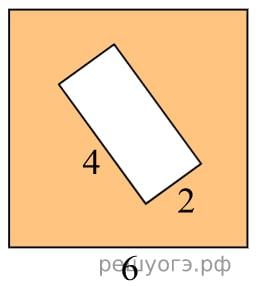
\includegraphics[align=t, width=\textwidth]{pics/G91M4L7-1}
	\end{minipage}
		\item Найдите площадь квадрата, описанного вокруг окружности радиуса \( 83 \).
		\item Найдите площадь прямоугольника, если его периметр равен \( 60 \), а отношение соседних сторон равно \( 4:11 \).
		\item В прямоугольнике одна сторона равна \( 96 \), а диагональ равна \( 100 \). Найдите площадь прямоугольника.
		\item 
		\begin{minipage}[t]{0.57\textwidth}
			Найдите площадь параллелограмма, изображённого на рисунке.
		\end{minipage}
		\begin{minipage}[c]{0.3\textwidth}
			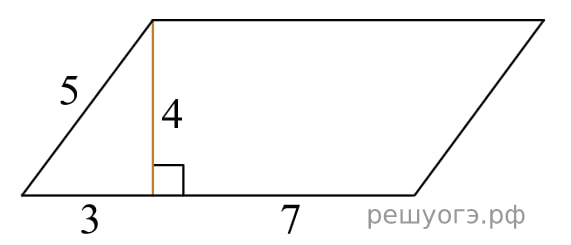
\includegraphics[align=t, width=\textwidth]{pics/G91M4L7-2}
		\end{minipage}
		\item Периметр ромба равен \( 24 \), а синус одного из углов равен \( \dfrac{1}{3} \). Найдите площадь ромба.
		\item В ромбе сторона равна \( 10 \), одна из диагоналей --- \( 5(\sqrt{6}-\sqrt{2})\), а угол, лежащий напротив этой диагонали, равен \( 30\degree \). Найдите площадь ромба.
		\item Найдите площадь ромба, если его диагонали равны \( 14 \) и \( 6 \).
		\item Высота \( BH \) параллелограмма \( ABCD \) делит его сторону \( AD \) на отрезки \( AH  =  1 \) и \( HD  =  28 \). Диагональ параллелограмма \( BD \) равна \( 53 \). Найдите площадь параллелограмма.
		\item В треугольнике одна из сторон равна \( 10 \), а опущенная на нее высота --- \( 5 \). Найдите площадь треугольника.
		\item В треугольнике одна из сторон равна \( 10 \), другая равна \( 10 \sqrt{3} \), а угол между ними равен \( 60\degree \). Найдите площадь треугольника.
		\item В треугольнике \( ABC \) отрезок \( DE \) --- средняя линия. Площадь треугольника \( CDE \) равна \( 97 \). Найдите площадь треугольника \( ABC \).
		\item Периметр треугольника равен \( 50 \), одна из сторон равна \( 20 \), а радиус вписанной в него окружности равен \( 4 \). Найдите площадь этого треугольника.
		\item Найдите площадь прямоугольного треугольника, если его катет и гипотенуза равны соответственно \( 28 \) и \( 100 \).
		\item Периметр равностороннего треугольника равен \( 30 \). Найдите его площадь, делённую на \( \sqrt{3} \).
		\item Периметр равнобедренного треугольника равен \( 16 \), а боковая сторона --- \( 5 \). Найдите площадь треугольника.
		\item 
		\begin{minipage}[t]{0.57\textwidth}
			Найдите площадь трапеции, изображённой на рисунке.
		\end{minipage}
		\begin{minipage}[c]{0.3\textwidth}
			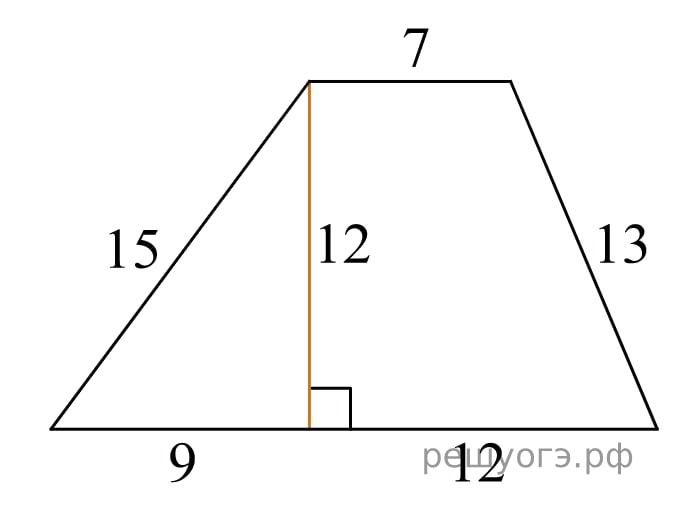
\includegraphics[align=t, width=\textwidth]{pics/G91M4L7-3}
		\end{minipage}
		\item Основания трапеции равны \( 18 \) и \( 12 \), одна из боковых сторон равна \( 6 \), а синус угла между ней и одним из оснований равен \( \dfrac{1}{3} \). Найдите площадь трапеции.
		\item 
	\end{listofex}
\end{class}
%
%===============>>  Провечная работа  <<===============
%
%\begin{exam}
%	\begin{listofex}
%	
%	\end{listofex}
%\end{exam}